\pagebreak
\section{Architectural Design}
 
\subsection{Overview}
Starting from a very general depiction of the overall system, the document explains in detail each component, through several class and component diagrams. In addition to this, a deployment view representing the physical implementation of myTaxiService and a description of the main patterns and styles used are provided. Please refer to each subsection for more details.

\newpage
\subsection{High level components and their interaction}
The overall system is divided in 5 macrocomponents. Please note that this is just a logical division (for example there are no classes entirely dedicated to the DB, since multiple Entity JavaBeans are used throughout each component). The main interactions between the components are briefly illustrated: for a more complete description please refer to section \ref{sub:component_interfaces}. For a detailed description of each component please refer to section \ref{sub:component_view} instead.


    \includegraphics[width=0.9\textwidth]{HighLevelArch}


\newpage
\subsection{Component view}
\label{sub:component_view}
The whole architecture can be described from two different points of view: 
\begin{itemize}
	\item \textbf{Tier division}: description of each tier, as given in section \ref{sec:deploy}.
	\item \textbf{Functionality}: each component represents a logical collection of correlated classes in the system (either representing data or business rules).
\end{itemize}

\newpage
\subsubsection{Client} % (fold)
Here are contained all classed related to a customer. In particular, two managers (one for guests and one for registered users) and an entity describing a Client are present. Whenever a guest/customer wants to do something strictly related to themselves (e.g. signing up, logging in..) he has to refer to this component.
\begin{figure}[hb]
    \centering
    \includegraphics[width=0.9\textwidth]{CompClassClient}
\end{figure}
% paragraph client (end)
        
\newpage
\subsubsection{TaxiRes} % (fold)
This component is responsible for two main objects in the entire system, Calls and Rides. A call is either a request or a reservation made by a customer, whereas a Ride describes the effective ride by a Taxi and can be associated with multiple calls. Whenever an action involves one of these classes, this is the component that must be used.
\vfill
\begin{figure}[hb]
    \centering
    \makebox[\textwidth][c]{\includegraphics[width=1.2\textwidth]{CompClassTaxiRes}}% 
\end{figure}
\vfill
% paragraph taxires (end)
        
\newpage
\subsubsection{TaxiAllocation} % (fold)
This is a central component for the service, since it is responsible for the actual allocation of a taxi for a certain ride. It holds a daemon always refreshing the ride queue to be processed by the DB and any TaxiHandler created by it.
\begin{figure}[h!]
    \centering
    \includegraphics[width=0.9\textwidth]{CompClassTaxiAlloc}
\end{figure}
% paragraph taxiallocation (end)

\newpage
\subsubsection{TaxiDriver} % (fold)
This component hold any information about taxis registered in the system and any action related to them (for example, updating the position of a cab according to the GPS data).
\begin{figure}[hb]
    \centering
    \includegraphics[width=0.9\textwidth]{CompClassTaxiDriver}
\end{figure}

\newpage
\subsubsection{DB} % (fold)
\label{par:db}
This is a logical component representing a layer between every other logic business and the DB. In order to better represent the structure of the DB supporting this service, a ER diagram is provided. As already said, each interaction with the database is mediated through Entity Java Beans, better described in section \ref{sub:component_view}.
\begin{figure}[h!]
    \centering
    \includegraphics[width=0.9\textwidth]{ER}
\end{figure}
% paragraph db (end)

\newpage
\subsection{Deployment view}
\label{sec:deploy}
% TODO 1= diagramma deployment
% 2 descrizione di ogni parte del deployment

\newpage
\subsection{Runtime view}
Since the actual representation of processes and threads running within myTaxiService would have been quite complex and difficult to explain, no runtime unit diagrams have been used. As shown in the algorithm section (\ref{sec:algorithm}), there is however something important on this point: TaxiAllocationDaemon and TaxiHandler work in a similar way to SocketManager and Socket. In fact, TaxiAllocationDaemon \emph{listens} to new rides through a repeated fetch operation on the DB and allocates a new TaxiHandler to manage one ride at a time.

Nevertheless, in order to catch the behaviour of the overall system, here are presented the improved sequence diagrams, better explaining what happens \emph{inside the box}.

\newpage
\subsubsection{Sign in} % (fold)
% xxx
\begin{figure}[h!]
    \centering
    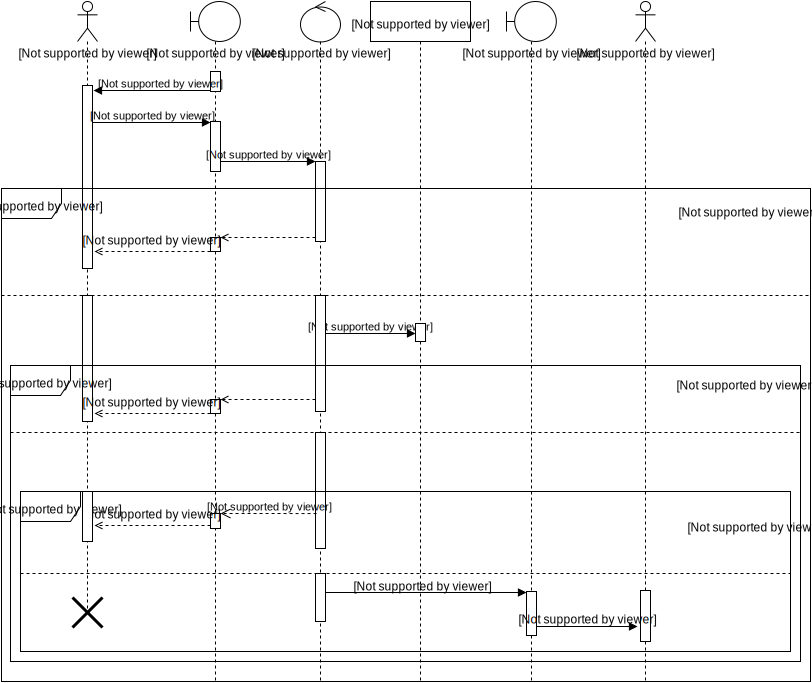
\includegraphics[width=0.9\textwidth]{SequenceSignIn}
\end{figure}

\newpage
\subsubsection{Sign up} % (fold)
% xxx
\begin{figure}[h!]
    \centering
    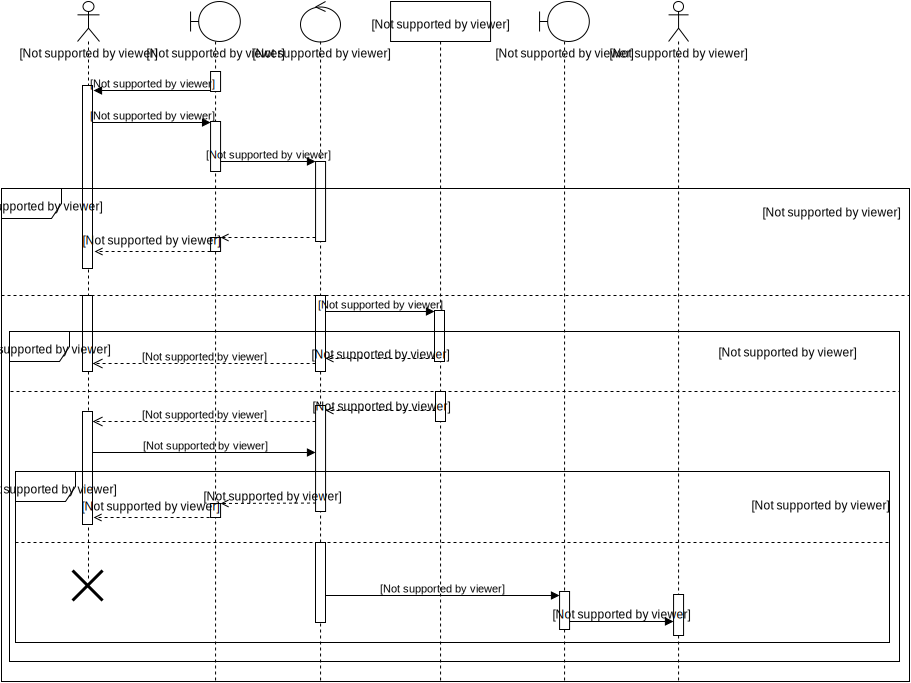
\includegraphics[width=0.9\textwidth]{SequenceSignUp}
\end{figure}

\newpage
\subsubsection{Allocate a taxi} % (fold)
% xxx
\begin{figure}[h!]
    \centering
    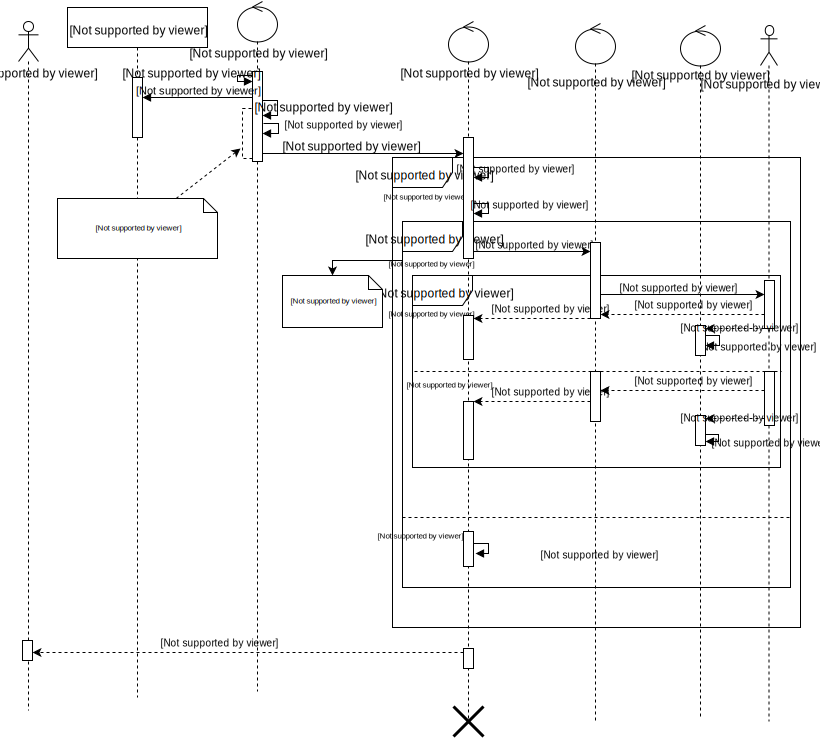
\includegraphics[width=0.9\textwidth]{SequenceAllocateTaxi}
\end{figure}

\newpage
\subsubsection{Request a taxi} % (fold)
% xxx
\begin{figure}[h!]
    \centering
    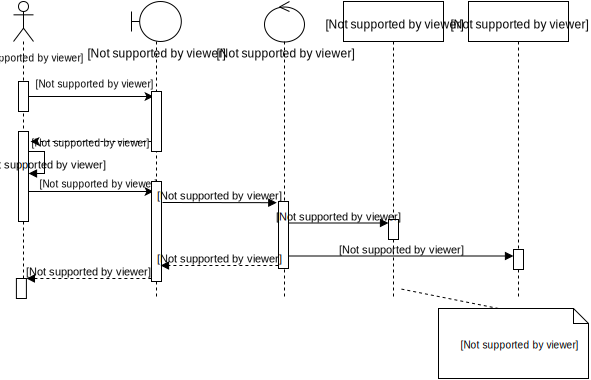
\includegraphics[width=0.9\textwidth]{SequenceRequestTaxi}
\end{figure}

\newpage
\subsubsection{Reserve a taxi} % (fold)
% xxx
\begin{figure}[h!]
    \centering
    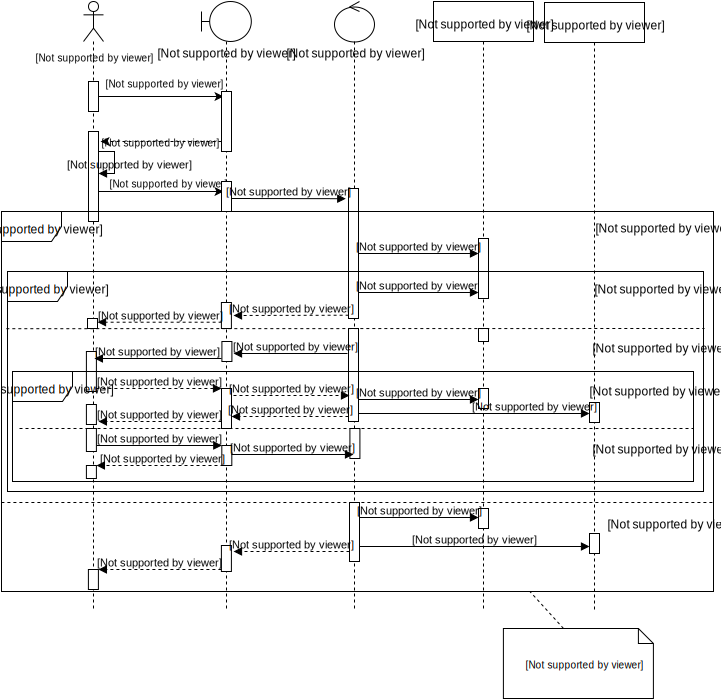
\includegraphics[width=0.9\textwidth]{SequenceReservation}
\end{figure}

\newpage
\subsubsection{Delete reservation} % (fold)
% xxx
\begin{figure}[h!]
    \centering
    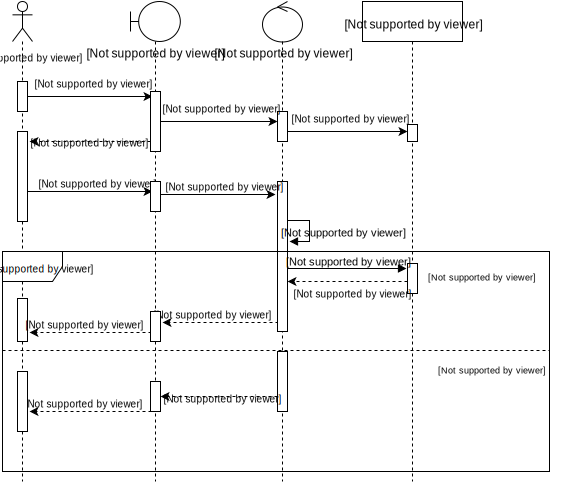
\includegraphics[width=0.9\textwidth]{DeleteReservation}
\end{figure}

\newpage
\subsection{Selected architectural styles and patterns}
This section describes high level patterns we decided to use in myTaxiService.

\paragraph{Deployment} A four-tier architecture is used in this project.
The whole infrastructure is divided in the following tiers:

\begin{itemize}
    \item{\textbf{Client tier} which is composed of web browsers and mobile app.}
    \item{\textbf{Presentation tier} whose aim is to generate user interface and send it to clients.}
    \item{\textbf{Logic tier} which coordinates the application: performs calculation, makes logical decisions and moves data between Presentation tier and Data tier.}
    \item{\textbf{Data tier} mainly made of entity beans and database. 
    Here information is stored and retrieved.}
\end{itemize}

We choose to use this kind of architecture because it provides a model by which
we can create a flexible and scalable system.

\paragraph{Communication} We choose to use a Service-oriented Architecture, 
an architecture which provides application functionality as a set of services, 
and applications that use those software services. 

Services are \textit{loosely coupled} units of functionality that are self-contained, 
Each service is an implementation of some interfaces, which provide a communication schema with
each application. Also, interfaces can be published and invoked.

\paragraph{Structure} Here we choose to use the Object-Oriented Architectural Style.
This is a design paradigm based on the division of responsibilities for a complex system
into small and reusable parts called ``Objects''.
They communicate with each other through interfaces, by sending and receiving messages
or by calling methods in other objects.

The main benefits of this approach are that it is:

\begin{itemize}
    \item{\textbf{Extensible} because there are a lot of structures which ensures that a change of implementation does not imply a change of interface.}
    \item{\textbf{Reusable} if each object should be developed as a reusable small piece of code.}
    \item{\textbf{Testable} because of the incapsulation, which improves testability.}
    \item{\textbf{Understandable} because it maps the application more closely to the real world.}
\end{itemize}

\newpage
\subsection{Component interfaces}
\label{sub:component_interfaces}

\subsubsection{Connection client - web server} % (fold)
\label{ssub:https}
The connection through the website to the service is guaranteed through standard HTTPS requests and are not described in detail here.
% subsubsection https (end)

\subsubsection{Connection application server - DB} % (fold)
\label{ssub:connection_application_server_db}
The application server uses EntityBeans to map relations into Java objects, which themselves refer to the underlying DB through JDBC calls. Since these connections are pretty standard (i.e. connection, query, handling results), they are not described in detail here.
% subsubsection connection_application_server_db (end)

\subsubsection{Web Service: JAX-WS} % (fold)
\label{ssub:web_service_jax_ws}
All public methods are available through a Web service, which is handled by JAX-WS on the server side. This means that each client knowing the address of the service can use it according to the functions described in detail below. Authorization for specific operations is controlled by tokens, as it is required in the parameter list.
% API PUBBLICA PUBBLICA (nel senso accessibile anche da esterno??) => WSDL

\newpage
\paragraph{Guest Manager} % (fold)
\label{par:guest_manager}
The GuestManager bean is responsible for operations on unregistered users; it let customers register, sign in or confirm their email after signing up.
\begin{table}[h!]
\centering
\resizebox{1\textwidth}{!}{
\begin{tabular}{llllll}
\toprule
    \textbf{Method name}		&	\textbf{Token} 	&	\textbf{User} 	&	\textbf{Parameter Name} 	& \textbf{Parameter Description} 	& \textbf{Returns} \\
    \midrule
    \multirow{3}{*}{signup} 			& 	\multirow{3}{*}{NO}		&	\multirow{3}{*}{Guest}	&	Username			&	Username for this customer			& True if operation succedeed \\
    									&							&							& Password			& Password for this customer \\
    									&							&							& Mail			& Mail for this customer \\\cmidrule{1-6}
    \multirow{2}{*}{login} 			& 	\multirow{2}{*}{NO}		&	\multirow{2}{*}{Guest}	&	Username			&	Username chosen during signup 			& Access token \\
    									&							&							& Password		& Hashed password for this user \\\cmidrule{1-6}
    \multirow{2}{*}{confirmEmail} 			& 	\multirow{2}{*}{NO}		&	\multirow{2}{*}{Customer}	&	Token			&	Mail token sent during registration			& Boolean response \\
    									&							&							& Mail		& Mail to be confirmed \\
    \bottomrule
\end{tabular}}
\end{table}
% paragraph guestmanager (end)

\paragraph{Customer Manager} % (fold)
\label{par:customer_manager}
The CustomerManager bean is responsible ????
\begin{table}[h!]
\centering
\resizebox{1\textwidth}{!}{
\begin{tabular}{llllll}
\toprule
    \textbf{Method name}		&	\textbf{Token} 	&	\textbf{User} 	&	\textbf{Parameter Name} 	& \textbf{Parameter Description} 	& \textbf{Returns} \\
    \midrule
    
%	\multirow{3}{*}{editProfile} 			& 	\multirow{3}{*}{YES}		&	\multirow{3}{*}{Customer}	&	Username			&	New username 			& Boolean response \\
%    									&							&							& Password		& New password \\
%    									&							&							& Payment Method		& New payment method (POS or cash) \\\cmidrule{1-6}
%    \multirow{2}{*}{deleteProfile} 			& 	\multirow{2}{*}{YES}		&	\multirow{2}{*}{Customer}	&	Username			&	Username chosen during signup 			& - \\
%    									&							&							& Password		& Password for this username \\\cmidrule{1-6}
     getPreviousRides 			& 	YES		&	Customer	&	Page			&	Page number of rides (10 rides per page)			& List of rides \\\cmidrule{1-6}
     
     logout 			& 	YES		&	-	&	-			&	-			& - \\
    \bottomrule
\end{tabular}}
\end{table}
% paragraph taxiresmanager (end)

\paragraph{TaxiResManager} % (fold)
\label{par:taxiresmanager}
TaxiResManager is responsible for the management of any call (aka request or reserve).

\begin{table}[h!]
\centering
\resizebox{1\textwidth}{!}{
\begin{tabular}{llllll}
\toprule
    \textbf{Method name}		&	\textbf{Token} 	&	\textbf{User} 	&	\textbf{Parameter Name} 	& \textbf{Parameter Description} 	& \textbf{Returns} \\
    \midrule
    \multirow{7}{*}{addCall} 			& 	\multirow{7}{*}{YES}		&	\multirow{7}{*}{Customer}	&	dateTime			&	When the call was made			& - \\
                                        &                           &                           & rideDateTime            & When the ride starts \\
    									&							&							& startPoint			& Starting point in associated ride \\
    									&							&							& endPoint			& Ending point in associated ride \\
    									&							&							& nrPeople			& How many seats are reserved \\
                                        &                           &                           & ???            & NON MI RICORDO PIU!!! \\
    									&							&							& paymentMethod			& POS / Cash \\\cmidrule{1-6}

    showCalls          &   YES     &   Customer    &   -          &   -        & Array of calls by this customer \\\cmidrule{1-6}
    removeCall 			& 	YES		&	Customer	&	IDCall			&	Call ID in DB table			& - \\
    									
    \bottomrule
\end{tabular}}
\end{table}
% paragraph customer_manager (end)

% \paragraph{RideManager} % (fold)
% \label{par:ridemanager}
% RideManager is responsible for any action involving a ride: adding one when a call is added to the DB, modifying one when something changes (for example, a new client in a shareable ride), deleting one or setting a new status for it.

% \begin{table}[h!]
% \centering
% \resizebox{1\textwidth}{!}{
% \begin{tabular}{llllll}
% \toprule
%     \textbf{Method name}        &   \textbf{Token}  &   \textbf{User}   &   \textbf{Parameter Name}     & \textbf{Parameter Description}    & \textbf{Returns} \\
%     \midrule
%     \multirow{4}{*}{addRide}            &   \multirow{4}{*}{YES}        &   \multirow{4}{*}{System} &       IDRide      &       Ride ID     & - \\
%                                         &                           &                           & startTime         & When the ride starts \\
%                                         &                           &                           & nrPeople          & Total number of people for this taxi \\
%                                         &                           &                           & expectedFee           & Fee calculated in advance for each customer \\\cmidrule{1-6}

%     removeRide          &   YES     &   System  &   IDRide          &   Ride ID in DB table         & - \\\cmidrule{1-6}

%     \multirow{4}{*}{updateRide}             &   \multirow{4}{*}{YES}        &   \multirow{4}{*}{System} &       RideID      &       Ride ID     & - \\
%                                         &                           &                           & nrPeople      & New total number of people  \\
%                                         &                           &                           & expectedFee       & New expected fee  \\
%                                         &                           &                           & endTime       & When the ride ends (optional)  \\\cmidrule{1-6}

%     \multirow{2}{*}{setStatus}          &   \multirow{2}{*}{YES}        &   \multirow{2}{*}{Systen} &   IDRide          &   Ride ID             & - \\
%                                         &                           &                           & Status        & New status for this ride \\\cmidrule{1-6}
    
%     getRideInfo             &   YES     &   System  &   IDRide          &   Ride ID in DB table         & Ride Info \\

%     \bottomrule
% \end{tabular}}
% \end{table}
% % paragraph ridemanager (end)

\paragraph{TaxiDriverManager} % (fold)
\label{par:taxidrivermanager}
TaxiDriverManager is responsible for the management of a single taxi driver through his own app.

\begin{table}[h!]
\centering
\resizebox{1\textwidth}{!}{
\begin{tabular}{llllll}
\toprule
    \textbf{Method name}		&	\textbf{Token (Taxi)} 	&	\textbf{User} 	&	\textbf{Parameter Name} 	& \textbf{Parameter Description} 	& \textbf{Returns} \\
    \midrule
    setAvailabilityStatus 			& 	YES		&	Taxi Driver / System	&	Status	& New status for this taxi & - \\\cmidrule{1-6}

    updatePosition			& 	YES		&	Taxi Driver	&	GPSCoords			&	Current GPS Coordinates for taxi		& - \\\cmidrule{1-6}

    setRideComplete          &   YES     &   Taxi Driver &   rideID           &   ID for current ride       & - \\
    									
    \bottomrule
\end{tabular}}
\end{table}
% paragraph taxidrivermanager (end)

% \paragraph{TaxiAllocationDaemon} % (fold)
% \label{par:taxiallocationdaemon}
% This is a Singleton JavaBean, responsible for allocating a taxi for each ride when necessary. It also holds all the Queues, divided by zone, for fast access.

% \begin{table}[h!]
% \centering
% \resizebox{1\textwidth}{!}{
% \begin{tabular}{llllll}
% \toprule
%     \textbf{Method name}		&	\textbf{Token} 	&	\textbf{User} 	&	\textbf{Parameter Name} 	& \textbf{Parameter Description} 	& \textbf{Returns} \\
%     \midrule
%     \multirow{2}{*}{createTaxiHandler} 			& 	\multirow{2}{*}{YES}		&	\multirow{2}{*}{System}	&		IDRide		&		Ride ID		& - \\
%     									&							&							& queue			& Queue for that zone \\\cmidrule{1-6}

%     deququeRide 			& 	YES		&	System	&	-			&	-			& Next ride to process \\\cmidrule{1-6}
    
%     refreshRideQueue 			& 	YES		&	System	&	-			&	-			& - \\

%     \bottomrule
% \end{tabular}}
% \end{table}

% paragraph taxiallocationdaemon (end)

% subsubsection web_service_jax_ws (end)
\newpage
\subsection{Other design decisions}

There are two aspects of myTaxiService we haven't discussed yet: communication 
with smartphones and geolocalization.

\paragraph {Mobile communication}
We need to send instant notifications to 
user or taxi's mobile devices. There is a standard way to do this, 
which is the one we have chosen, \textit{Push Notification}.

We decided to support both iOS and Android smartphones. In order to send push
notifications to iOS smartphone, we have to use \textit{Apple Push Notification Service}.
The same applies to Android world, Google has its own push service, called 
\textit{Google Cloud Messaging}.

\paragraph {Geolocalization}
We decided to use Google Maps as geolocalization service because it is highly
reliable, fast and extremely used in the world.
Also, it offers powerful APIs which allow us to use it for a wide variety of use cases.
